\section{Cost Analysis and Comparison}
\label{sec:cost-analysis}

% ---------------------------------------------------------------
%  PARAGRAPH 1: THE FUNDAMENTAL TRADEOFF
% ---------------------------------------------------------------

The passage from standard QSP to its stereographic variant
replaces one cost with another.  In the standard framework, the
signal value $a = r/\alpha$ is normalized to $[-1,1]$ by dividing
by $\alpha \geq \|H\|$, and this normalization factor propagates
through the circuit: the total depth scales as
$\mathcal{O}(d \cdot \alpha)$, where $d$ is the polynomial degree
and $\alpha$ can be large.  Stereographic encoding avoids this
normalization entirely---the signal $r \in [0,\infty)$ enters as
$\rtilde = r/\sqrt{1+r^2} \in [0,1)$, and the circuit depth depends
only on~$d$, not on~$\|H\|$.  The saving is not free: the Bloch
sphere becomes increasingly compressed near the north pole as
$r$ grows, and recovering the encoded value from measurements
requires resolving ever-smaller differences in Pauli expectation
values.  The coherent normalization overhead of standard QSP
reappears as a classical sampling overhead in the stereographic
approach.

% ---------------------------------------------------------------
%  PARAGRAPH 2: ERROR PROPAGATION — developed as a narrative
% ---------------------------------------------------------------

To quantify this overhead, consider the stereographic decoding
formula~\eqref{eq:decoding}, which recovers the encoded value~$z$
from the ratio
$\langle\PauliX\rangle/(1 - \langle\PauliZ\rangle)$.
As $r \to \infty$, the denominator
$1 - \langle\PauliZ\rangle \to 0$: the Bloch vector approaches
the north pole, and its projection onto the equatorial plane
carries progressively less information.  A first-order error
propagation (Appendix~\ref{app:proofs}) shows that if each Pauli
expectation is estimated with precision~$\delta$, the decoded
value $\hat{z}$ satisfies
\begin{equation}
	|\hat{z} - z| \leq \frac{(1+r^2)(1+r)}{2}\,\delta.
	\label{eq:error-bound}
\end{equation}
The error amplification grows as $r^3$ for large~$r$: the
numerator measurement contributes $\mathcal{O}(r^2)$ and the
denominator measurement $\mathcal{O}(r^3)$.  Since each Pauli
expectation estimated from $N$ shots has precision
$\delta = \mathcal{O}(1/\sqrt{N})$, achieving absolute precision
$|\hat{z} - z| \leq \epsilon$ requires
\begin{equation}
	N = \mathcal{O}\!\left(\frac{(1+r^2)^2(1+r)^2}{\epsilon^2}\right) = \mathcal{O}\!\left(\frac{r^6}{\epsilon^2}\right) \quad \text{for } r \gg 1.
	\label{eq:shot-count}
\end{equation}
For \emph{relative} precision
$|\hat{z}/z - 1| \leq \epsilon_{\mathrm{rel}}$, the scaling
improves to
\begin{equation}
	N = \mathcal{O}\!\left(\frac{r^4}{\epsilon_{\mathrm{rel}}^2}\right) \quad \text{for } r \gg 1,
	\label{eq:shot-count-rel}
\end{equation}
since the relative error bound is
$|\delta z/z| \leq (1+r^2)(1+r)/(2r)\,\delta$, which grows as
$r^2$ rather than $r^3$.  The crucial point is that the overhead
is \emph{polynomial} in~$r$, not exponential: large eigenvalues
are expensive to decode, but not catastrophically so.

% ---------------------------------------------------------------
%  PARAGRAPH 3: CONVERGENCE RATES — Boyd's theory (from PDF)
% ---------------------------------------------------------------

The sampling cost quantifies one half of the resource budget; the
other half is the polynomial degree~$d$ required to approximate the
target function.  Here the stereographic framework connects
directly to the classical approximation theory of Boyd's rational
Chebyshev functions~\cite{Boyd1990,Boyd1987}.  The composition of a
target function $f(r)$ with the inverse stereographic map
$r = \rtilde/\sqrt{1-\rtilde^2}$ yields a function of
$\rtilde \in (-1,1)$ whose rational Chebyshev expansion converges
at a rate determined by the analytic structure of~$f$.  Boyd
identifies two regimes~\cite{Boyd1990}: for functions that are
analytic in a neighborhood of the real axis and decay algebraically
at infinity---the \emph{geometric convergence class}---the
Fourier--Chebyshev coefficients decay as
$|a_k| \leq C\exp(-qk)$ for some $q > 0$, so that $L^\infty$-error
$\epsilon$ is achieved at degree $d = \mathcal{O}(\log(1/\epsilon))$.
For functions that are entire but have essential singularities at
$|y| \to \infty$---the \emph{subgeometric class}---the coefficients
decay more slowly, typically as $\exp(-c\sqrt{k})$, and the required
degree grows as $d = \mathcal{O}(\log^2(1/\epsilon))$.  In either
case, convergence is guaranteed on the full real line without any
domain truncation, a property that distinguishes the stereographic
approach from standard Chebyshev approximations on a rescaled
compact interval $[-L,L]$, which require a truncation parameter~$L$
growing with the problem size.

% ---------------------------------------------------------------
%  PARAGRAPH 4: SPECIFIC FUNCTION CLASSES — concrete rates
% ---------------------------------------------------------------

These rates make precise the polynomial degree entering the circuit
depth.  The Lorentzian $f(r) = 1/(1+r^2)$, which arises in
Cauchy distributions and resonance profiles, provides the most
striking example: composing with the stereographic map yields
$f(\rtilde/\sqrt{1-\rtilde^2}) = 1 - \rtilde^2$, a degree-2
polynomial, so no approximation is needed at all.  More
generally, generalized Lorentzians $1/(1+r^2)^s$ map to
$(1-\rtilde^2)^s$, a polynomial of degree~$2s$.  For the
hyperbolic secant $\operatorname{sech}(r)$, the pullback to
the circle is $C^\infty$ with all derivatives vanishing at the
endpoints, and the nearest singularity of
$\operatorname{sech}(z)$ to the real axis (at $z = i\pi/2$)
controls the Fourier decay rate: the result is geometric
convergence at degree $d = \mathcal{O}(\log(1/\epsilon))$.
Gaussian targets $\exp(-\beta r^2/2)$, by contrast, are entire
but produce essential singularities at $\theta = 0, \pi$ after
pullback to the circle, so their Fourier coefficients decay only
subgeometrically, giving $d = \mathcal{O}(\log^2(1/\epsilon))$.
For any rational function $P(r)/Q(r)$ with $\deg Q > \deg P$ and
no real poles, the convergence is geometric, with the degree
controlled by the distance of the nearest complex pole from the
real axis.  These rates apply to both the eigenvalue
transformation setting of this section and to the state
preparation application of Section~\ref{sec:applications}.

% ---------------------------------------------------------------
%  PARAGRAPH 5: EIGENVALUE INVERSION — case study
% ---------------------------------------------------------------

Eigenvalue inversion illustrates the depth-versus-sampling
tradeoff most concretely.  The function
$f(\lambda) = 1/\lambda$ is central to quantum linear-systems
algorithms~\cite{HHL2009,ChildsWiebe2012} and is a natural
testbed for stereographic QSP because $1/\lambda$ diverges as
$\lambda \to 0$---precisely the kind of unbounded function that
standard QSP cannot realize directly.  In the standard
framework, one normalizes $H \to H/\alpha$ with
$\alpha \geq \|H\|$, then approximates $f(a) = 1/(\alpha a)$
by a bounded polynomial of degree
$\mathcal{O}(\kappa\log(1/\epsilon))$, where
$\kappa = \alpha/\lambda_{\min}$ is the condition number; the
resulting circuit depth is
$\mathcal{O}(\alpha\kappa\log(1/\epsilon))$.  In the
stereographic framework, the target in the bounded variable is
\begin{equation}
	\frac{P(a)}{Q(a)} = \frac{1}{r} = \frac{\sqrt{1-a^2}}{a},
	\label{eq:inversion-target}
\end{equation}
where $a = \rtilde = \lambda/\sqrt{1+\lambda^2}$.  No
normalization constant appears: the target
$\sqrt{1-a^2}/a$ is a ratio of the Chebyshev
components at $d = 2$, so the QSP degree required is
minimal.  The query depth is
$\mathcal{O}(d)$ independent of $\|H\|$, at the cost of a
sampling overhead scaling as
$\mathcal{O}(\lambda_{\max}^6/\epsilon^2)$ for absolute
precision.  We emphasize that the single-qubit analysis
characterizes the approximation quality in the compressed
variable; the extension to eigenvalue transformations of a
multi-qubit Hamiltonian requires the stereographic block
encoding developed in the companion
paper~\cite{KharaziLeytonOrtega2026b}.  For operators where
$\|H\|$ is large but the eigenvalues of interest are moderate,
the depth saving can be substantial.

% ---------------------------------------------------------------
%  PARAGRAPH 6: TARGET GALLERY — numerical evidence
% ---------------------------------------------------------------

Figure~\ref{fig:target-gallery} provides numerical evidence for
the convergence theory across four representative target functions:
eigenvalue inversion $1/r$, the Lorentzian $1/(1+r^2)$, the
inverse square root $1/\sqrt{1+r^2}$, and the Gaussian
$e^{-r^2}$.  In each case, the decoded ratio
$P(\rtilde)/Q(\rtilde)$ tracks the exact target increasingly
well as the QSP degree~$d$ increases.  The pointwise error
reveals the spatial structure of the approximation: for $1/r$,
errors are concentrated at small $r$ where the target diverges;
for the bounded targets, errors are spread more uniformly.
Eigenvalue inversion is the most favorable case---the $d = 2$
base case already achieves errors below $10^{-7}$---while the
bounded targets require higher degree, consistent with the
algebraic convergence expected when the stereographic map
introduces branch points at $\rtilde = \pm 1$.  The inset
in panel~(e) summarizes the maximum approximation error versus
degree for all four targets, confirming that eigenvalue inversion
converges fastest while bounded targets converge more slowly.

\begin{figure*}[tp]
	\centering
	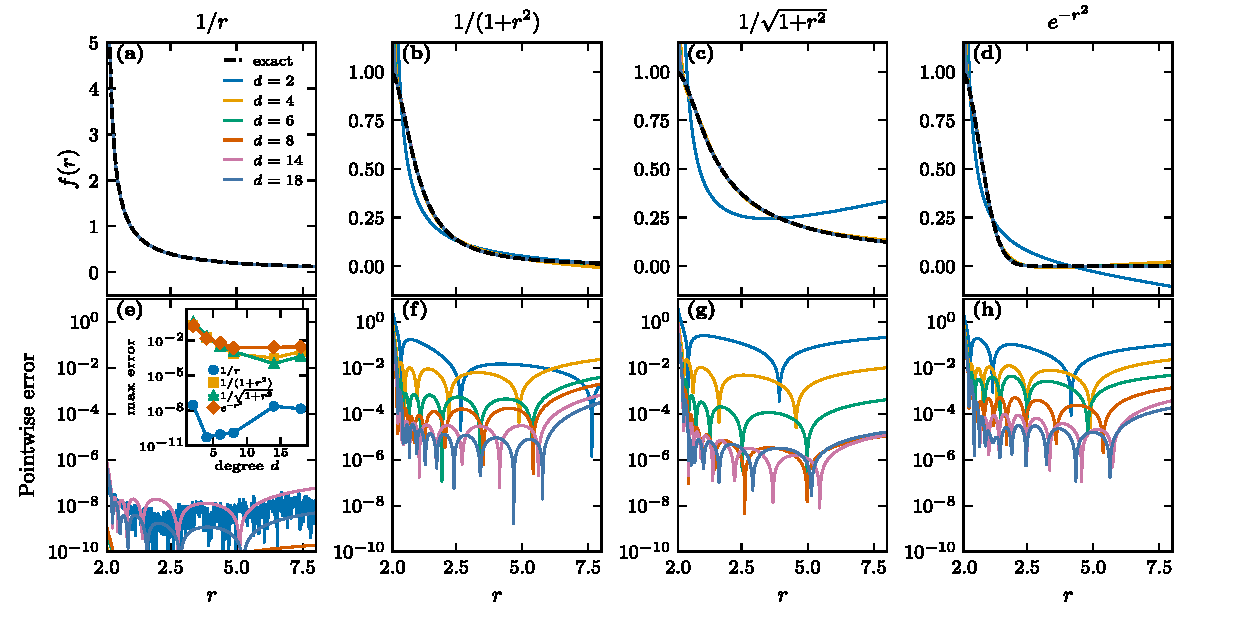
\includegraphics[width=\textwidth]{figures/target_gallery.pdf}
	\caption{Stereographic QSP approximation of four target functions. \emph{Top row}~(a--d): decoded rational functions $P(\rtilde)/Q(\rtilde)$ (colored lines, one color per QSP degree~$d$; see legend in~(a)) compared to the exact target (dashed black). All approximations improve systematically with increasing degree. \emph{Bottom row}~(e--h): pointwise error $|f_d(r) - f(r)|$ on a logarithmic scale. For eigenvalue inversion (a,~e), errors are below $10^{-7}$ even at low degree because the $d=2$ base case already captures $1/r$. For the bounded targets (b--d, f--h), the error decreases with degree but more slowly, reflecting the branch point at $\rtilde = \pm 1$. \emph{Inset} in~(e): maximum approximation error on the fitting interval versus QSP degree~$d$ for all four targets, showing that eigenvalue inversion converges fastest while bounded targets converge more slowly.}
	\label{fig:target-gallery}
\end{figure*}

% ---------------------------------------------------------------
%  PARAGRAPH 7: HEAD-TO-HEAD COMPARISON — the table
% ---------------------------------------------------------------

Table~\ref{tab:cost-comparison} collects the structural comparison
of the three QSP frameworks.  The stereographic approach is the
only variant whose output range is unbounded, a direct consequence
of the rational decoding; it is also the only one whose circuit
depth is independent of the operator norm~$\alpha$.  These
advantages come at the cost of a sampling overhead that grows
polynomially with the largest eigenvalue, and a requirement that
the eigenbasis be known for the multi-qubit extension.  GQSP
shares the $\mathcal{O}(d)$ depth scaling but retains the
boundedness constraint and requires normalization, while standard
QSVT carries the full $\mathcal{O}(d \cdot \alpha)$ depth but
needs no eigenbasis knowledge and incurs only $\mathcal{O}(1/\epsilon^2)$
sampling cost.

\begin{table*}[t]
	\caption{Cost comparison of standard, stereographic, and generalized QSP approaches for implementing a function $f(\lambda)$ of the eigenvalues of a Hermitian operator $H$. Here $\alpha = \|H\|$, $\kappa$ is the condition number, $d$ is the polynomial degree, and $r = \max_j |\lambda_j|$ is the maximum eigenvalue magnitude.  ``Queries'' counts calls to the block encoding or signal unitary; in standard QSP/QSVT the required degree~$d$ itself depends on~$\alpha$ through the normalization (e.g., $d = \mathcal{O}(\alpha\kappa\log(1/\epsilon))$ for eigenvalue inversion).}
	\label{tab:cost-comparison}
	\begin{ruledtabular}
		\begin{tabular}{llll}
			                     & Standard QSP/QSVT                   & Stereographic QSP                     & GQSP~\cite{MotlaghWiebe2023}              \\
			\hline
			Output constraint    & $|P(a)| \leq 1$ on $[-1,1]$         & $|P(\rtilde)|^2 + |Q(\rtilde)|^2 = 1$ & $|P(e^{i\theta})| \leq 1$ on $\mathbb{T}$ \\
			Output range         & Bounded                             & Unbounded (rational)                  & Bounded                                   \\
			Queries              & $d$ ($d$ depends on $\alpha$)        & $d$ ($d$ independent of $\alpha$)     & $d$                                       \\
			Ancilla qubits       & $\geq 1$ (implementation-dependent) & $1$                                   & $1$                                       \\
			Normalization        & Required ($\alpha \geq \|H\|$)      & Not required                          & Required ($\alpha \geq \|H\|$)            \\
			Sampling cost        & $\mathcal{O}(1/\epsilon^2)$         & $\mathcal{O}(r^6/\epsilon^2)$         & $\mathcal{O}(1/\epsilon^2)$               \\
			Input domain         & $a \in [-1,1]$                      & $r \in [0,\infty)$                    & $e^{i\theta} \in \mathbb{T}$              \\
			Eigenbasis knowledge & Not required                        & Required (multi-qubit)                & Not required                              \\
			Polynomial parity    & Required                            & Required                              & Not required                              \\
		\end{tabular}
	\end{ruledtabular}
\end{table*}

% ---------------------------------------------------------------
%  PARAGRAPH 8: THE NATURAL REGIME — when to use each
% ---------------------------------------------------------------

The interplay between convergence rate and sampling cost identifies
the natural regime for each approach.  When the eigenvalues of
interest satisfy $r = \mathcal{O}(1)$, the stereographic sampling
overhead is $\mathcal{O}(1/\epsilon^2)$---the same as standard
QSP---and the depth saving of eliminating the factor of~$\alpha$
is obtained for free; for depth-limited devices where circuit
fidelity degrades rapidly with gate count, this can be the
decisive advantage.  For operators whose eigenvalues span a wide
range including $r \gg 1$, the $\mathcal{O}(r^6/\epsilon^2)$
sampling cost becomes prohibitive, and standard QSVT---which pays
$\mathcal{O}(\alpha)$ coherently but has constant sampling
cost---is preferable.  The stereographic framework is also
particularly well suited to genuinely unbounded target functions
($1/\lambda$, $\lambda$, $\tan\lambda$) that standard QSP can
only approximate after truncation and regularization, and to
structured Hamiltonians with a known eigenbasis where the
multi-qubit extension applies directly.
Section~\ref{sec:applications} develops an application of
stereographic QSP to quantum state preparation, showing how the
rational Chebyshev convergence rates translate into concrete gate
complexity bounds.  Section~\ref{sec:discussion} discusses the
relationship to standard QSP/QSVT and generalized QSP in more
detail.
